\chapter{GeneroCity}

In questo capitolo verrà descritta l'applicazione di GeneroCity e in particolar modo come i sensori operano in essa. Verrà prima delineata la sua architettura generale per poi approfondire i dettagli implementativi riguardanti l'integrazione dei sensori nell'applicazione per Android. 

\section{L'architettura dell'applicazione}
L'applicazione di Generocity è basata su un'architettura di tipo client-server\footnote{Il sistema client-server è un'architettura di rete dove un dispositivo terminale o client si connette ad un server per usufruire di un servizio.} ed è quindi divisa in due componenti principali tra loro interconnesse: il \textit{backend} e il \textit{frontend}. Queste due componenti comunicano tra di loro utilizzando il protocollo HTTP\footnote{HTTP, acronimo di HyperText Transfer Protocol, è il principale protocollo di livello applicativo usato per il trasferimento di dati sul web.}.

\subsection{Backend}
Il backend è il software che si occupa dell'effettiva elaborazione dei dati e di gestire il database al fine di immagazzinarli e accedere ad essi. Esso espone delle funzionalità attraverso una web API\footnote{Una API, acronimo di Application Software Interface, è un tipo di interfaccia software che permette ad un programma di offrire servizi e funzionalità ad altri software.}, definendo come le altre componenti software devono interagire con il server senza la necessità di condividere codice sorgente ma effettuando delle richieste HTTP a degli specifici URL chiamati endpoint.
\begin{figure}[h]
    \centering
    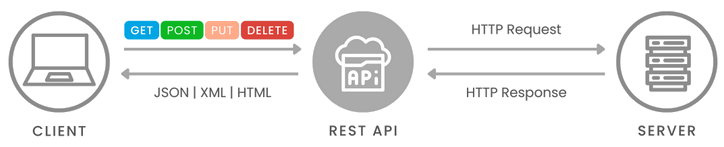
\includegraphics[width=1\linewidth]{images/rest.png}
    \caption{Comunicazione tramite API REST}
    \label{fig:rest}
\end{figure}
In particolare il backend di GeneroCity adotta una filosofia REST, la quale definisce una serie di principi chiave per la progettazione progettazione di una API.


\subsection{Frontend}
Il frontend invece è il programma con cui l'utente finale interagisce direttamente, in questo caso attraverso un'interfaccia grafica. Questa componente invierà le richieste agli endpoint definiti dal backend per inviare e ottenere dei dati. Esistono due versioni
\begin{wrapfigure}[23]{r}{0.4\textwidth}
    \centering
    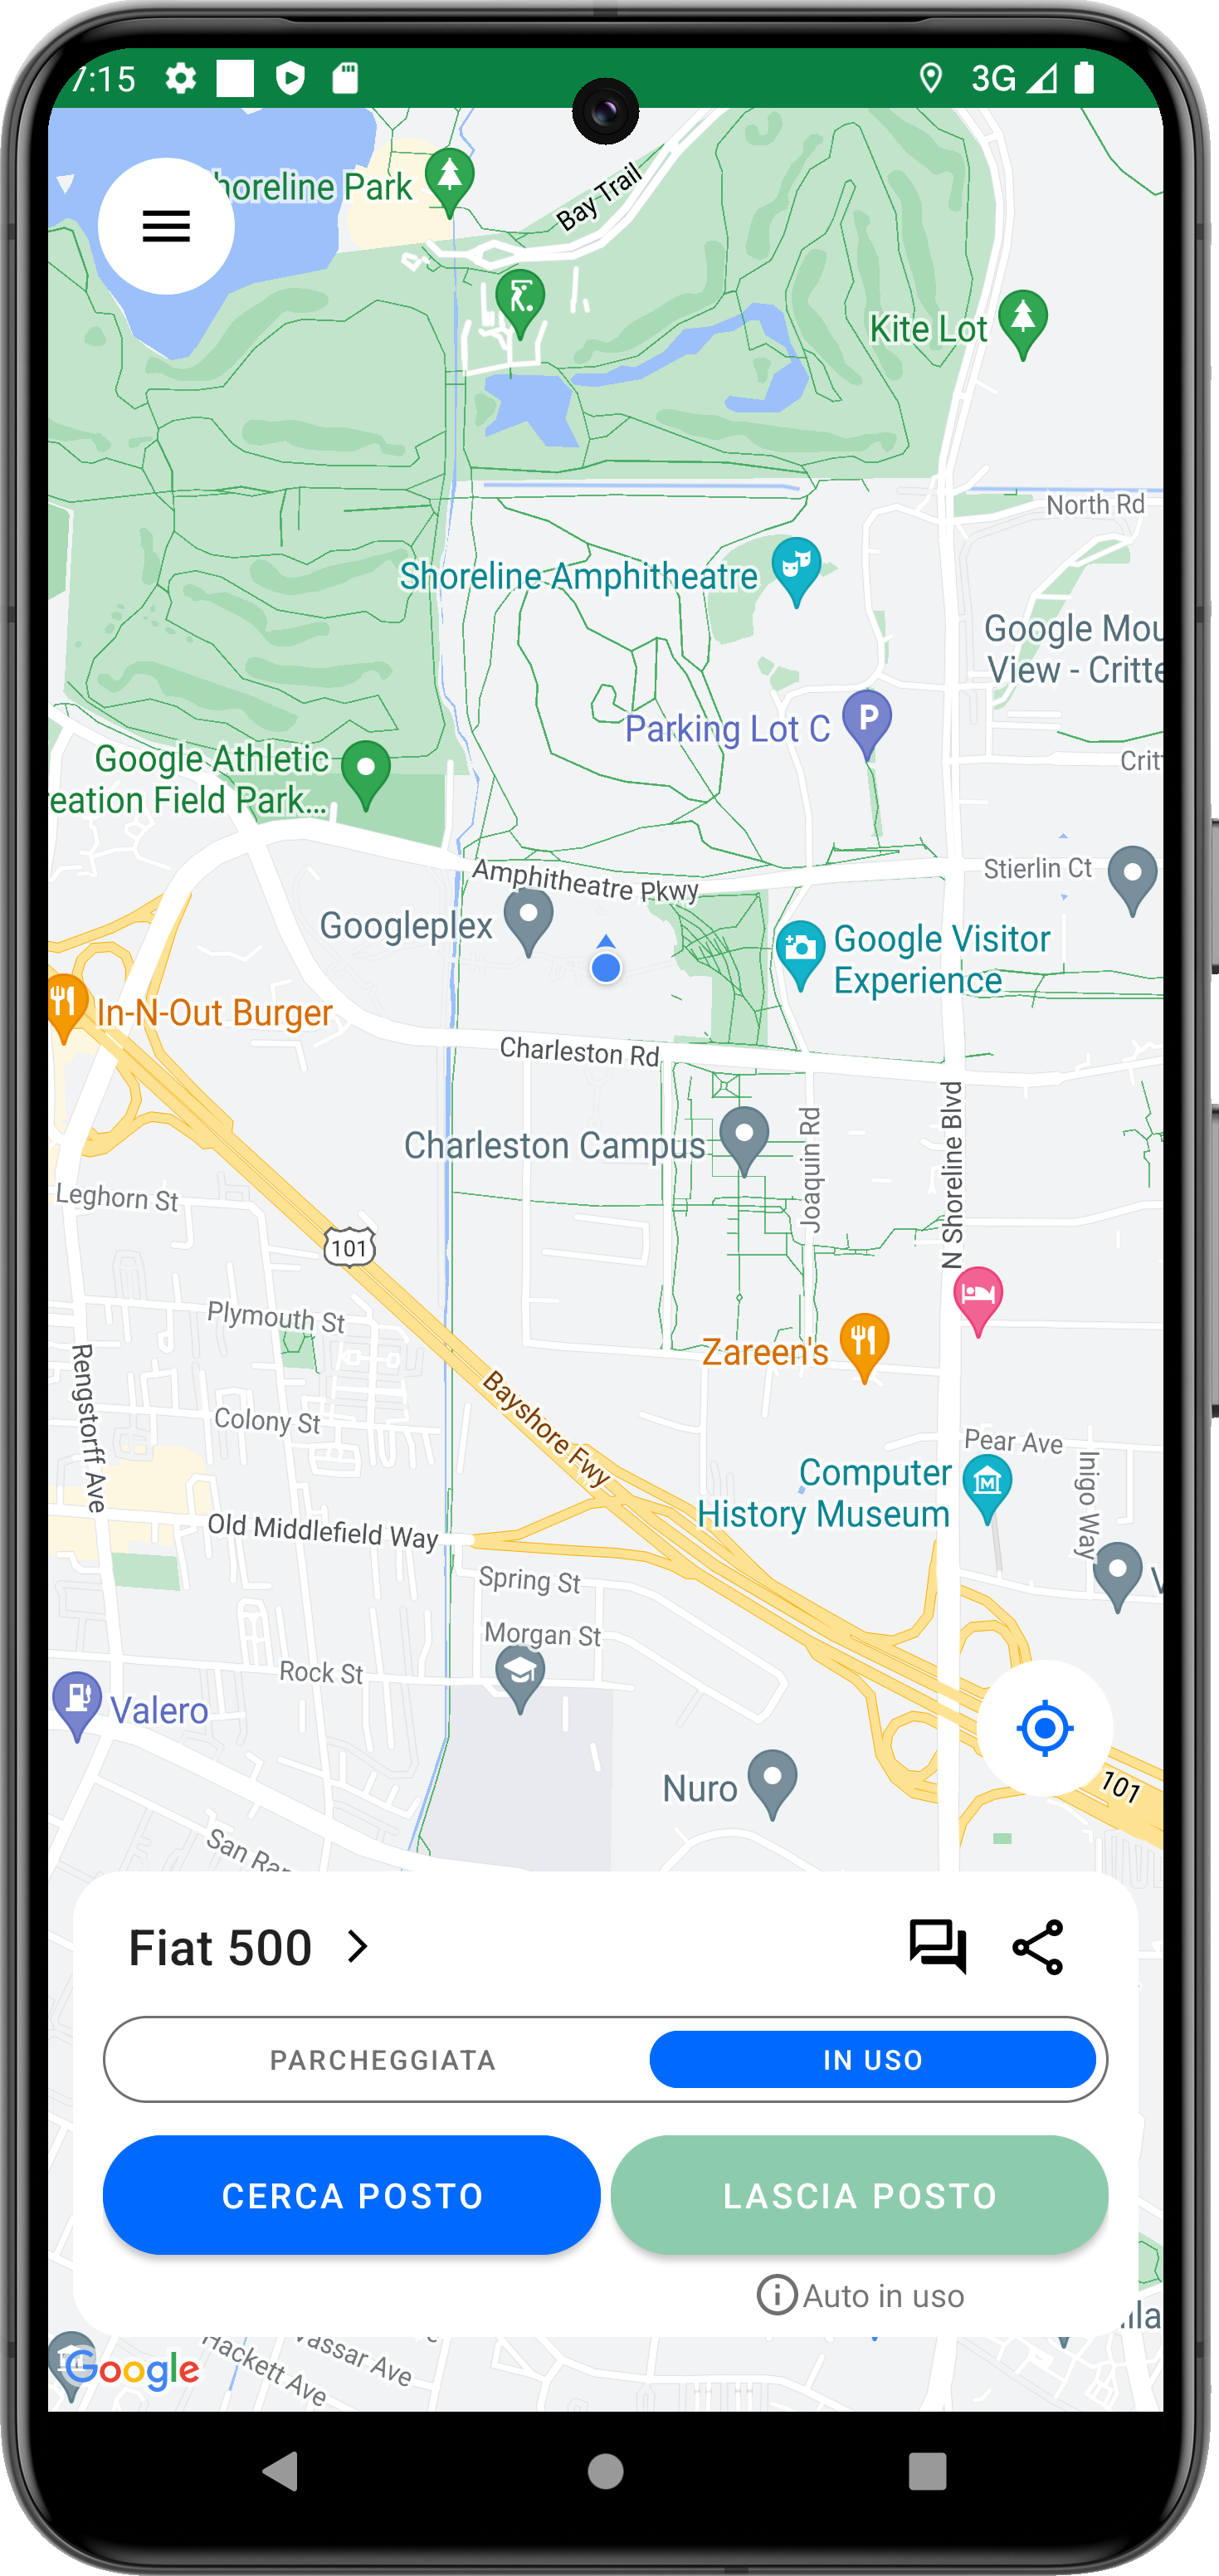
\includegraphics[width=0.9\linewidth]{images/gc_main_activity.png}
    \caption{GeneroCity Android}
    \label{fig:main_screen}
\end{wrapfigure}
differenti del frontend di Generocity: un'applicazione per Android scritta in Java e una in Swift per iOS. Si è scelto di sviluppare due applicazioni in maniera nativa anziché utilizzare un approccio cross-platform\footnote{Con cross-platform si intende un'applicazione che viene sviluppata una sola volta con un unico codice sorgente, ma può essere eseguita su diversi sistemi operativi. Si differisce dall'approccio il quale prevede l'utilizzo di un linguaggio di programmazione specifico per la piattaforma utilizzata.} a causa dell'estensivo utilizzo di funzionalità di sistema che verrà fatto dai sensori.

La loro gestione, infatti,  avviene interamente nel frontend e richiede che il loro funzionamento sia ben coordinato per garantire che lo stato dell'utente sia continuamente aggiornato. Di seguito verranno analizzati i dettagli implementativi riguardanti questo aggiornamento.


\section{Il flusso di aggiornamento della confidenza dei sensori}
Dato che in GeneroCity i sensori presenti sono molteplici, un fattore importante è la loro coordinazione: lo stato dell'utente sarà determinato basandosi sulla confidenza di ogni sensore ed è quindi importante che esso sia aggiornato ogni qualvolta un sensore cambia la sua confidenza. Per sincronizzare il lavoro dei sensori è stato quindi fondamentale definire delle funzionalità comuni che ogni sensore deve avere. Questo è stato possibile sfruttando il paradigma di programmazione orientata agli oggetti implementato in Java, in particolare è stata definita una classe astratta\footnote{Nella programmazione orientata agli oggetti una classe astratta è una classe che non può essere istanziata, la quale definisce delle funzionalità di base per tutte le sue sotto classi.} che tutti i sensori ereditano.

\subsection{La classe astratta Sensor}
Ogni sensore eredita dalla classe Sensor i seguenti attributi: il \textit{nome} univoco che identifica il sensore, la \textit{versione} del sensore, il \textit{peso} (rappresentato come numero reale) che ha il sensore nel calcolo dello stato dell'utente.

Inoltre ogni sensore mantiene uno storico della confidenza che ha calcolato tramite una mappa ad albero\footnote{Una treemap è una struttura dati che implementa le funzionalità di normale una normale mappa, ossia immagazzina delle coppie (chiave, valore), e inoltre mantiene l'ordinamento delle coppie basato sull'ordinamento naturale delle chiavi.} che adotta come chiave lo Unix Timestamp, ossia il numero di secondi trascorsi dalla mezzanotte del 1° Gennaio 1970, che indica il momento in cui il valore è stato calcolato. Di seguito vengono riportati i principali metodi esposti da questa classe.
\subsubsection{getStatus}
\begin{minted}[
framesep=2mm,
linenos,
bgcolor=LightGray,
breaklines
]{java}
public abstract double getStatus(Calendar timestamp);
\end{minted}
Esso ha come parametro un Timestamp e restituisce la confidenza del sensore calcolata nell'istante più vicino a quello passato come parametro. Questo metodo è l'unico metodo astratto ed è quindi il metodo principale che i sensori concreti dovranno implementare.
\subsubsection{update}

\begin{minted}[
framesep=2mm,
linenos,
bgcolor=LightGray,
breaklines
]{java}
public void update(Calendar timestamp, SensorData sensorData) {
    collect(timestamp, sensorData);
    GCSensorConstants.onUpdate(timestamp);
}
\end{minted}
Il metodo update riceve in input un Timestamp e un oggetto di un tipo da noi definito, denominato SensorData, contenente i dati inviati dal sensore. Questo metodo si occuperà di inviare i dati raccolti al server, attraverso il metodo \textit{collect}, e di innescare il ricalcolo dello stato dell'utente.
Quando viene eseguito il metodo update viene notificata l'unità centrale: una classe statica chiamata SensorConstants. Essa, attraverso il metodo \textit{onUpdate}, richiede lo stato di ogni sensore (utilizzando il metodo getStatus) e calcola il nuovo stato dell'utente attraverso il metodo \textit{compute}. Attualmente questo stato viene rappresentato come la media pesata delle confidenza di ogni sensore in uno specifico momento.

\subsubsection{GCSensorConstants.onUpdate}
\begin{minted}[
framesep=2mm,
linenos,
breaklines,
bgcolor=LightGray,
]{java}
static void onUpdate(Calendar time) {
    if (updating) {
        return;
    }

    updating = true;
    double computed = compute(time);
    computeHistory.put(time.getTimeInMillis(), computed);
    updating = false;
}
\end{minted}

\subsubsection{GCSensorConstants.compute}
\begin{minted}[
framesep=2mm,
linenos,
bgcolor=LightGray,
breaklines
]{java}
private static double compute(Calendar time) {
    double sum = 0.0;
    double wei = 0.0;

    double confidence;
    for (GCSensorInterface module : sensors) {
        confidence = module.getStatus(time);

        sum += (confidence - 0.5d) * module.weight;
        wei += module.weight;
    }

    return sum / wei + 0.5d;
}
\end{minted}

\subsection{L'invio di dati al server}
Come anticipato ogni qualvolta viene aggiornata la confidenza di un sensore il metodo update richiede in input un oggetto di tipo SensorData che rappresenta lo stato del sensore al momento dell'aggiornamento. Questo perché, prima che venga ricalcolata la confidenza media, viene chiamato il metodo \textit{collect} che serializza l'oggetto in formato JSON e lo invia al server tramite una richiesta HTTP all'endpoint in figura \ref{fig:endpoint}, il quale si occuperà di memorizzare i dati forniti dal sensore nel database. Questi dati vengono mantenuti al fine sia di tenere traccia del corretto funzionamento dei sensori, sia perché verranno utilizzati per l'allenamento di un modello di Machine Learning che verrà implementato in futuro in GeneroCity per determinare lo stato dell'utente.

\begin{figure}[h]
    \centering
    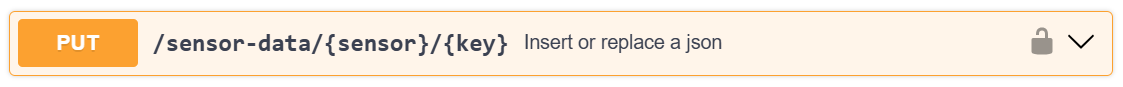
\includegraphics[width=1\linewidth]{images/endpoint.png}
    \caption{L'endpoint chiamato per memorizzare i dati dei sensori sul database}
    \label{fig:endpoint}
\end{figure}

\subsubsection{collect}
\begin{minted}[
framesep=2mm,
linenos,
bgcolor=LightGray,
breaklines
]{java}
public void collect(Calendar timestamp, SensorData sensorData) {
    long tsMillis = timestamp.getTimeInMillis();
    if (tsMillis - lastApiTimestamp <= getApiCooldownMs()) {
        return;
    }

    lastApiTimestamp = tsMillis;
    String key = ver + "-" + app.config().getMyId() + "-" + timestamp.getTimeInMillis();
    app.api().setSensorData(name, key, sensorData).enqueue(updateCall);
}
\end{minted}
La classe SensorData serializza le seguenti informazioni:
\begin{itemize}
    \item \textit{datetime}: la data e l'ora in cui è avvenuto l'aggiornamento seguendo il formato definito nello standard RFC3339\cite{ref:RFC3339};
    \item \textit{confidence}: la confidenza calcolata dal sensore al momento dell'aggiornamento;
    \item \textit{action}: l'azione che il sensore ha rilevato (\textit{walking}, \textit{unknown} o \textit{automotive});
    \item \textit{data}: alcuni dati aggiuntivi specifici del sensore che ha effettuato la rilevazione, i quali indicano lo stato in cui si trovava il sensore. Ad esempio per il sensore Wi-Fi questi dati possono essere relativi alla rete a cui il dispositivo è connesso, mentre per il sensore GPS le coordinate geografiche in cui l'utente si trova.
\end{itemize}
Di seguito un esempio di body inviato dal sensore bluetooth attraverso una richiesta HTTP:
\begin{minted}[
framesep=2mm,
linenos,
bgcolor=LightGray,
breaklines
]{json}
{
   "action":"automotive",
   "confidence":0.75436,
   "data":{
      "connected":[
         {
            "alias":"My Car",
            "bluetooth_class":"Handsfree",
            "connection_count":4,
            "device_name":"Fiat Punto",
            "is_car":true
         }
      ],
      "bluetooth_enabled":true
   },
   "datetime":"2024-10-21T15:43:24.525+02:00"
}
\end{minted}
Come si può notare il campo data è costruito sulla base dello stato del sensore: in particolare si evince che il bluetooth è attivo e il dispositivo è connesso ad un dispositivo che viene identificato come macchina.

In aggiunta a questi dati nel path della richiesta (figura \ref{fig:endpoint}) vengono anche mandati il nome del sensore utilizzato ed una chiave univoca usata per identificare la richiesta nel database. Essa è costruita utilizzando la versione del sensore, l'id dell'utente autenticato nell'applicazione ed il Timestamp del momento in cui viene inviata la richiesta.

Inoltre, onde evitare un sovraccarico del server, è stato definito un tempo di \textit{cooldown} tra le richieste: ogni volta che viene notificato un aggiornamento da parte del sensore, se questo tempo non è trascorso dall'ultima richiesta, allora la richiesta viene scartata ma viene comunque ricalcolata la nuova media.
